% JPM-style Beamer defense deck (30 minutes) — MSCI U.S. Equity Factors (2014–2026) + COVID-19 deep-dive
% Source of all quantitative claims: tables/figures generated in this project (CSV + figures in /mnt/data) and the companion paper (Extended_Equity_GARCH.tex).

\documentclass[10pt,aspectratio=169]{beamer}

% ---------- Theme (clean, JPM-friendly) ----------
\usetheme{metropolis}
\metroset{progressbar=frametitle,sectionpage=progressbar,numbering=fraction}

% ---------- Packages ----------
\usepackage[utf8]{inputenc}
\usepackage[T1]{fontenc}
\usepackage{amsmath,amsfonts,amssymb}
\usepackage{booktabs}
\usepackage{graphicx}
\usepackage{caption}
\usepackage{subcaption}
\usepackage{threeparttable}
\usepackage{siunitx}
\usepackage{xcolor}
\usepackage{hyperref}

% ---------- Helpers ----------
\newcommand{\sm}{\small}
\newcommand{\xs}{\scriptsize}
\newcommand{\xsp}{\scriptsize\vspace{2pt}}

\title{Asymmetric Volatility, Regime Dependence, and Tail-Risk Calibration in MSCI U.S. Equity Factors\\\vspace{2mm}\large Evidence from GARCH/EGARCH, VaR Backtests, and Conditional Mean--Variance Allocation}
\author{Youssef Louraoui}
\institute{youssef.louraoui@essec.edu}
\date{\today}

\begin{document}

% ========================
% Title
% ========================
\begin{frame}
  \titlepage
\end{frame}

% ========================
% Roadmap
% ========================
\begin{frame}{Roadmap}
\sm
\begin{enumerate}
  \item Motivation \& contribution: why volatility modeling is the bottleneck in factor risk
  \item Data \& stylized facts: non-normality, high correlations, and crisis co-movement
  \item Volatility modeling: GARCH vs EGARCH, leverage effects, persistence
  \item Regime dependence: conditional efficiency across volatility states
  \item Tail-risk calibration: 95\% vs 99\% VaR (Kupiec) and what fails in the extreme tail
  \item Portfolio construction: conditional covariance \(\Rightarrow\) frontier compression and ``diversification collapse''
  \item COVID-19 as a stress laboratory: linking asymmetry, correlation convergence, VaR rejection, and frontier compression
  \item Practical implications \& research extensions
\end{enumerate}
\end{frame}

% ========================
% 1. Motivation & contribution
% ========================
\section{Motivation \& Contribution}

\begin{frame}{Core question}
\sm
\textbf{When markets enter extreme volatility states, do standard symmetric volatility models (GARCH) mis-calibrate factor risk in a way that matters for allocation and VaR governance?}

\vspace{2mm}
\begin{itemize}
  \item The paper uses MSCI U.S. equity factor indices (Value, Momentum, Quality, MinVol, Size) and SPX as the market proxy.
  \item Empirical focus: (i) 2014--2026 ``full sample'' regime behavior; (ii) COVID-19 2019--2021 as an extreme-volatility case study.
  \item Output focus: volatility asymmetry (EGARCH), regime-conditioned efficiency, VaR backtesting, and conditional mean--variance allocation.
\end{itemize}
\end{frame}

\begin{frame}{Contributions}
\sm
\begin{enumerate}
  \item \textbf{Unified empirical narrative} linking four crisis mechanisms measured on the same factor universe:
    \begin{itemize}
      \item volatility asymmetry (EGARCH leverage),
      \item volatility persistence (half-life),
      \item correlation convergence in stress (dependence tightening),
      \item and \textbf{portfolio-level frontier compression} under conditional covariance.
    \end{itemize}
  \item \textbf{Governance-relevant diagnostics}: VaR passes at 95\% for most series but \emph{systematically fails at 99\%} (Kupiec), concentrating model risk where oversight is most stringent.
  \item \textbf{Actionable translation}: model-implied conditional covariance produces an investable allocation map (Equal Weight vs Vol Parity vs MinVar) that reveals when ``diversification'' becomes structurally constrained.
\end{enumerate}
\end{frame}

% ========================
% 2. Data & Stylized Facts
% ========================
\section{Data \& Stylized Facts}

\begin{frame}{Data, universe, and design}
\sm
\begin{itemize}
  \item Universe: SPX (market) + five MSCI U.S. factor indices: Momentum, Value, Quality, Minimum Volatility, Size.
  \item Frequency: daily returns. Horizon: 2014--2026 for the long-sample analysis; 2019--2021 for the COVID stress window.
  \item Modeling stack:
  \begin{itemize}
    \item univariate volatility: GARCH(1,1) and EGARCH(1,1),
    \item regime split by volatility state (Low/Med/High),
    \item tail calibration: dynamic VaR and Kupiec unconditional coverage,
    \item portfolio layer: conditional mean--variance cloud (5,000 long-only portfolios) under model-implied covariance.
  \end{itemize}
\end{itemize}
\end{frame}

\begin{frame}{Stylized fact \#1: Factor premia exist, but crisis co-movement is material}
\centering

\includegraphics[width=0.95\linewidth]{02_cum_returns.png}
% \xsp
% \xs\textit{Cumulative returns rebased to 1 (2014--2026). Source: project figure /mnt/data/02\_cum\_returns.png.}
\end{frame}

\begin{frame}{Stylized fact \#2: Unconditional correlations are high (diversification is limited ex ante)}
\centering
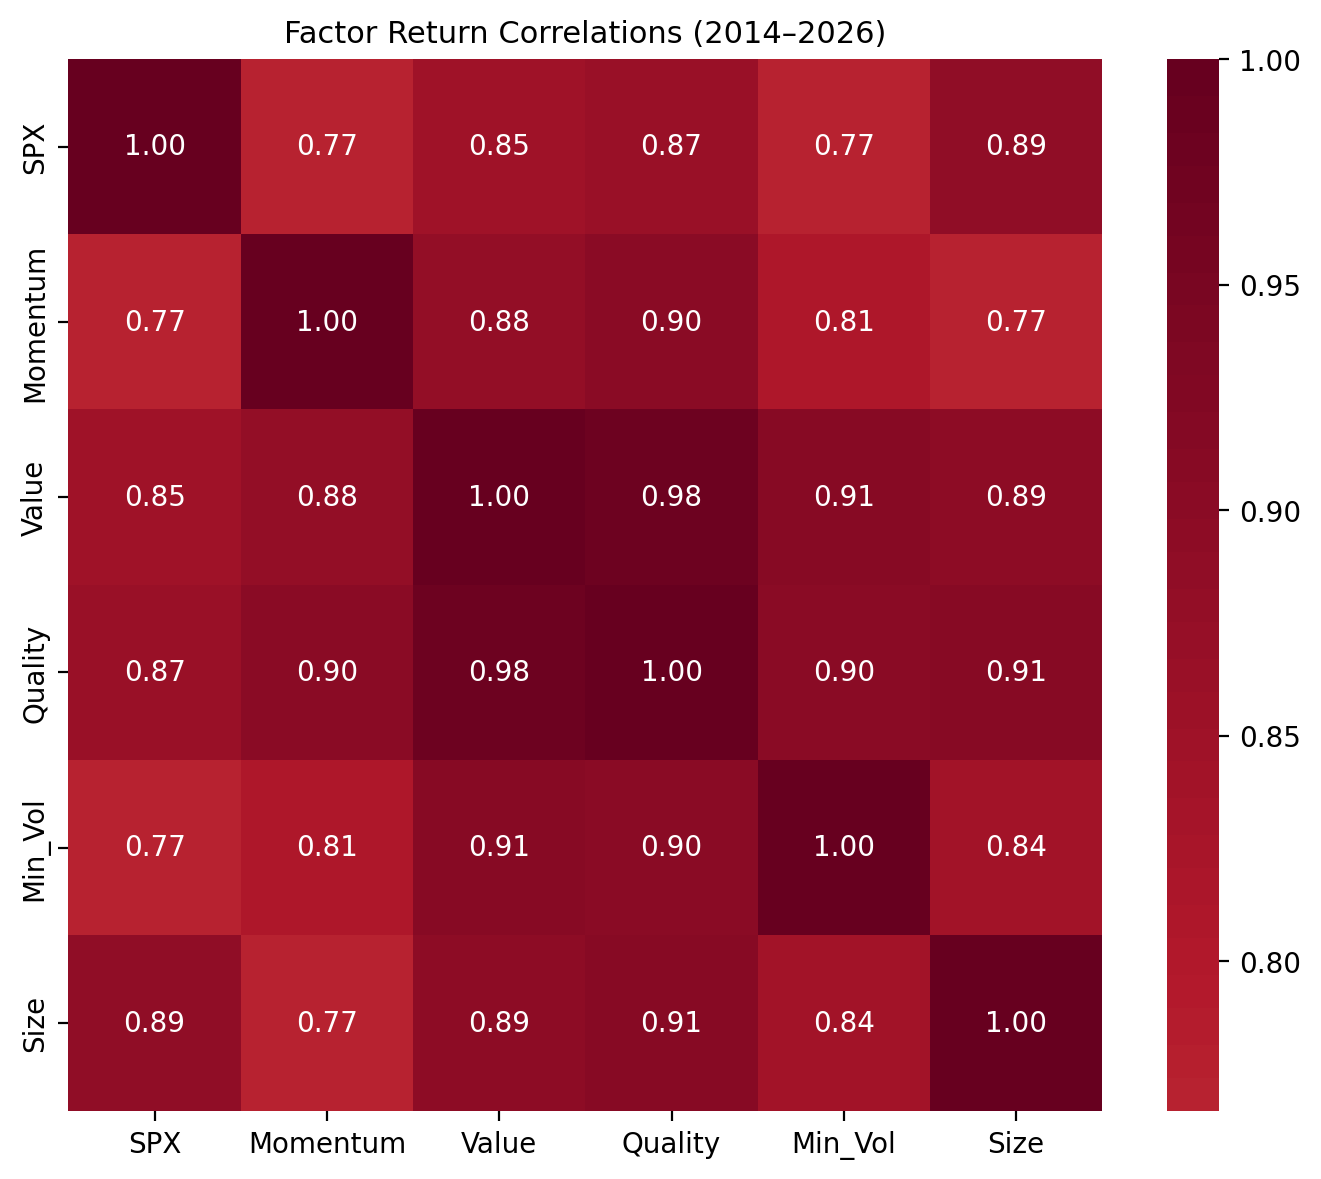
\includegraphics[width=0.50\linewidth]{03_corr_full.png}
\end{frame}

% ========================
% 3. Volatility modeling (GARCH vs EGARCH)
% ========================
\section{Volatility Modeling: GARCH vs EGARCH}

\begin{frame}{Modeling intuition (minimal math)}
\sm
\begin{columns}[T,onlytextwidth]
\column{0.52\textwidth}
\textbf{Symmetric GARCH(1,1)}
\begin{equation*}
\sigma_t^2=\omega+\alpha\varepsilon_{t-1}^2+\beta\sigma_{t-1}^2
\end{equation*}
\begin{itemize}
  \item Captures volatility clustering.
  \item Imposes \emph{symmetry}: \(+\varepsilon\) and \(-\varepsilon\) of same size have identical impact.
\end{itemize}

\column{0.48\textwidth}
\textbf{Asymmetric EGARCH(1,1)}
\begin{equation*}
\ln\sigma_t^2=\omega+\beta\ln\sigma_{t-1}^2+\alpha\Big(\tfrac{|\varepsilon_{t-1}|}{\sigma_{t-1}}-\mathbb{E}|z|\Big)+\gamma\tfrac{\varepsilon_{t-1}}{\sigma_{t-1}}
\end{equation*}
\begin{itemize}
  \item \(\gamma<0\): negative shocks increase volatility \emph{more} than positive shocks.
  \item Directly targets leverage/asymmetry documented in the empirical volatility literature.
\end{itemize}
\end{columns}
\end{frame}

\begin{frame}{Conditional volatility paths: GARCH vs EGARCH (2014--2026)}
\centering

\includegraphics[width=0.60\linewidth]{05_vol_overlay.png}
% \xsp
% \xs\textit{Conditional volatility estimates under GARCH and EGARCH for each series.}
\end{frame}

\begin{frame}{Asymmetry is systematic: News impact curves (GARCH vs EGARCH)}
\centering

\includegraphics[width=0.75\linewidth]{11_news_impact_curves.png}
\end{frame}

\begin{frame}{Persistence, half-life, and leverage (cross-factor summary)}
\sm
\textbf{Key empirical message:} GARCH persistence is high (slow mean reversion), while EGARCH leverage is negative across all series.
\vspace{2mm}
\begin{itemize}
  \item GARCH half-lives are measured in \emph{weeks}, not days.
  \item Leverage ranks are economically meaningful: Value/Quality show the largest negative \(\gamma\) in the project estimates.
\end{itemize}

\includegraphics[width=0.95\linewidth]{13_persistence_halflife_leverage.png}
\end{frame}

% ========================
% 4. Regimes
% ========================
\section{Volatility Regimes \& Conditional Efficiency}

\begin{frame}{Regime design and why it matters}
\sm
\begin{itemize}
\item \textbf{State variable.} Daily volatility regime is defined using the \emph{GARCH(1,1) conditional volatility} of the market sleeve (SPX proxy), $\hat{\sigma}_{t}^{\text{SPX}}$.
\item \textbf{Tercile classification.} Each day $t$ is assigned to:
\begin{align*}
\text{Low Vol} &: \hat{\sigma}_{t}^{\text{SPX}} \leq Q_{33} \\
\text{Medium Vol} &: Q_{33} < \hat{\sigma}_{t}^{\text{SPX}} \leq Q_{67} \\
\text{High Vol} &: \hat{\sigma}_{t}^{\text{SPX}} > Q_{67}
\end{align*}
where $Q_{33}$ and $Q_{67}$ are the 33rd and 67th percentiles of $\hat{\sigma}_{t}^{\text{SPX}}$ over the full sample.
\item \textbf{Within-regime diagnostics.} For each factor and regime, we compute mean return, volatility, a Sharpe proxy (mean/vol), and regime-specific max drawdown.
\item \textbf{Interpretation.} This design converts volatility persistence into economically meaningful ``states'' and provides an allocation-relevant lens: conditional efficiency and diversification are evaluated \emph{where the portfolio actually lives} (in regimes that persist for weeks, not days).
\end{itemize}
\end{frame}

\begin{frame}{Return distributions shift materially across regimes}
\centering

\includegraphics[width=0.75\linewidth]{12b_regime_return_distributions.png}
% \xsp
% \xs\textit{Return distributions by volatility regime (SPX-based classification). Source: /mnt/data/12b\_regime\_return\_distributions.png.}
\end{frame}

\begin{frame}{Conditional Sharpe proxy by regime (heatmap) + time spent in each regime}
\centering
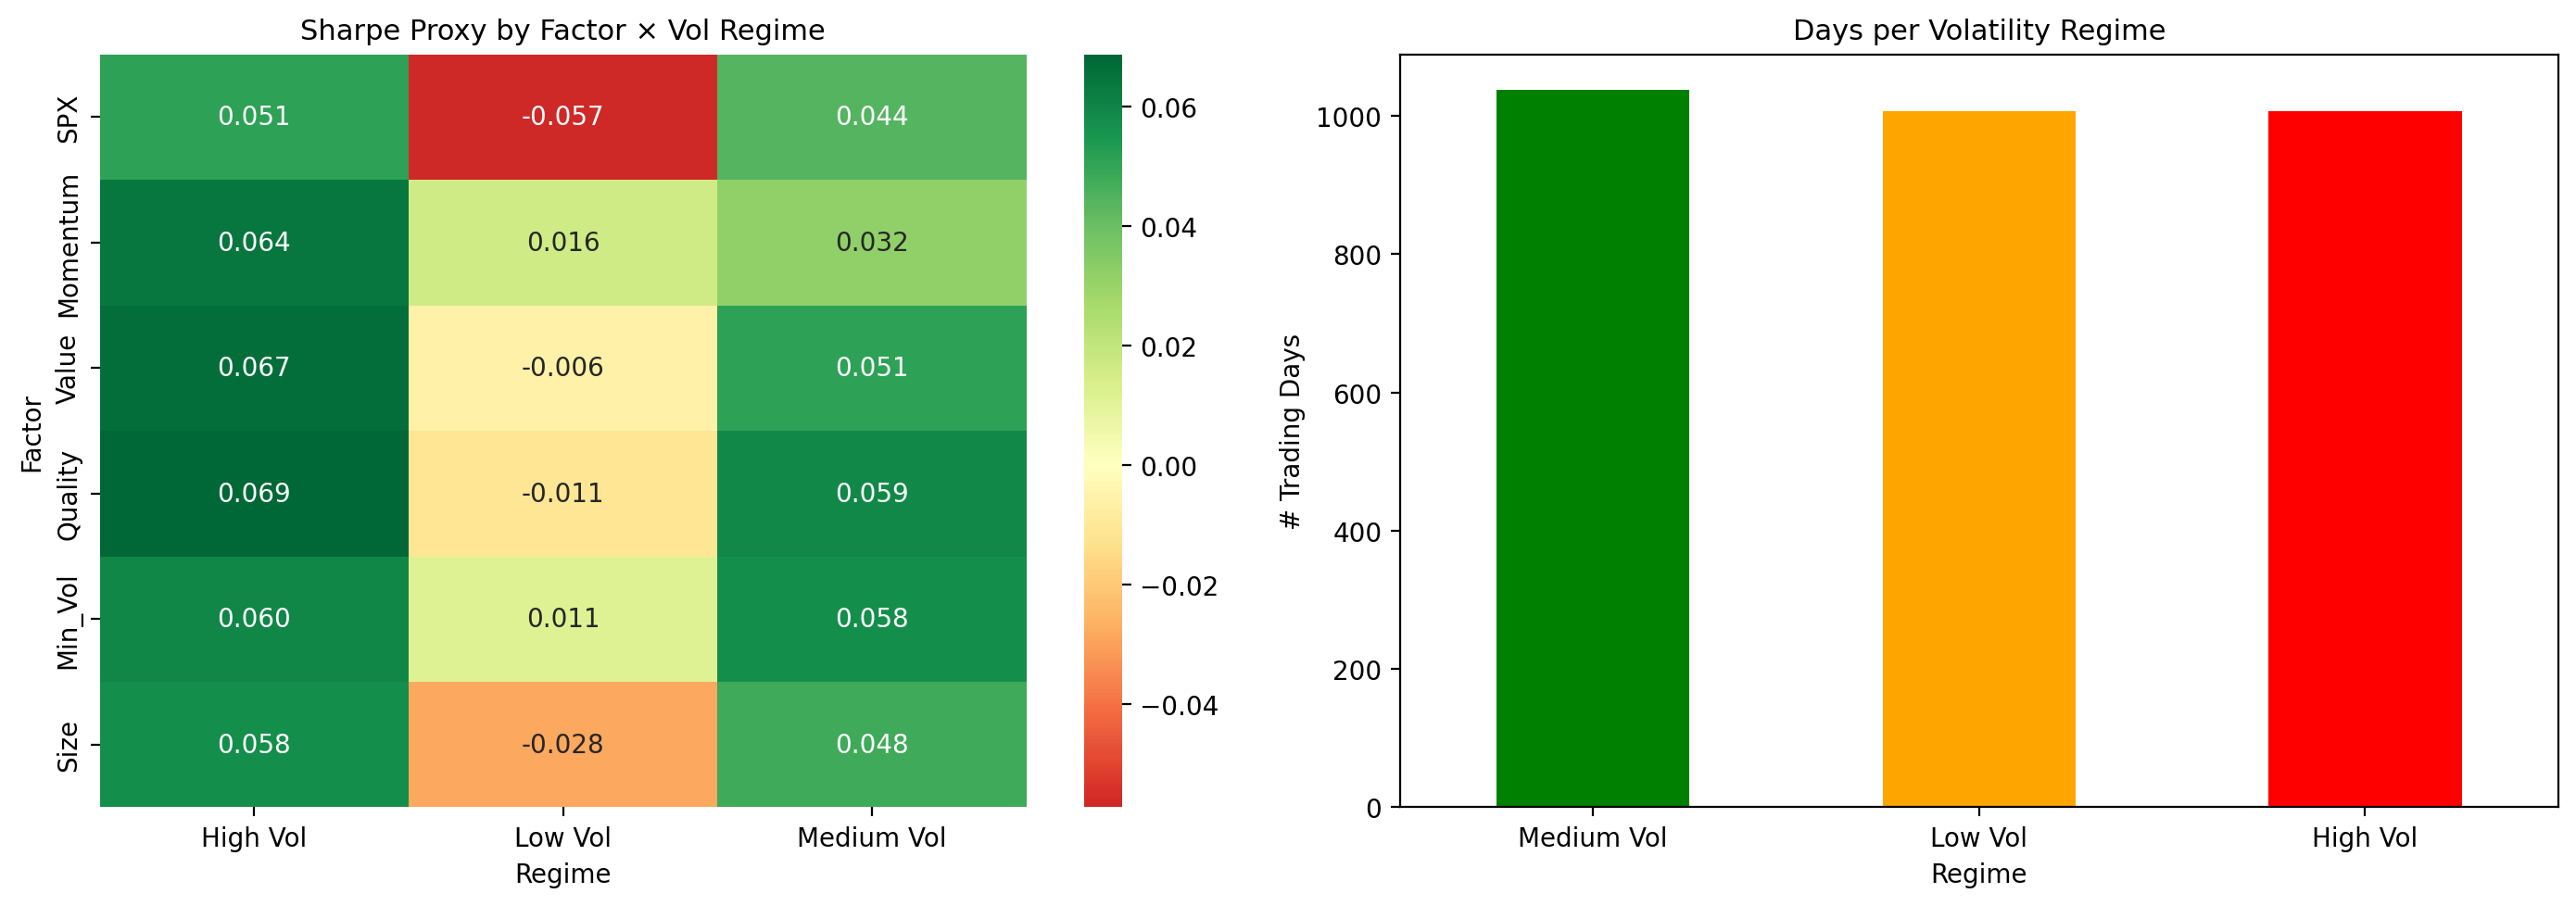
\includegraphics[width=0.95\linewidth]{12_vol_regime_analysis.png}
% \xsp
% \xs\textit{Sharpe proxy (mean/vol) by factor \(\times\) regime and days per regime. Source: /mnt/data/12\_vol\_regime\_analysis.png.}
\end{frame}

% ========================
% 5. Tail risk & VaR
% ========================
\section{Tail Risk Calibration: VaR Backtests}

\begin{frame}{Why VaR backtesting is the governance bottleneck}
\sm
\begin{itemize}
  \item Passing VaR at \(95\%\) is not informative about robustness at \(99\%\).
  \item The project’s Kupiec tests show that mis-calibration concentrates in the \emph{extreme} left tail.
  \item This is consistent with the paper’s descriptive evidence: fat tails + leverage + crisis clustering.
\end{itemize}
\end{frame}

\begin{frame}{Dynamic 99\% VaR backtest (SPX): GARCH vs EGARCH}
\centering

\includegraphics[width=0.95\linewidth]{10_var_backtest_spx.png}
% \xsp
% \xs\textit{Dynamic VaR exceedances and Kupiec p-values for SPX. Source: /mnt/data/10\_var\_backtest\_spx.png.}
\end{frame}

\begin{frame}{Kupiec unconditional coverage: 95\% vs 99\% (summary)}
\sm
\begin{columns}[T,onlytextwidth]
\column{0.5\textwidth}
\textbf{Panel A: 95\% VaR}
\begin{itemize}
  \item Breach rates cluster near 5\% for most factors.
  \item Momentum is the systematic exception (higher breaches and lower p-values).
\end{itemize}

\column{0.5\textwidth}
\textbf{Panel B: 99\% VaR}
\begin{itemize}
  \item Breach rates are \emph{materially above} 1\% across the universe under both models.
  \item EGARCH improves SPX coverage (higher p-value) but does not fully eliminate rejection.
\end{itemize}
\end{columns}

\vspace{2mm}
\xs\textit{Numbers shown on the next slide are extracted from the project CSV (VaR\_Backtest\_Kupiec.csv).}
\end{frame}

\begin{frame}{Kupiec VaR backtests (extracted from CSV)}
\sm
\begin{columns}[T,onlytextwidth]
\column{0.5\textwidth}
\textbf{Panel A: 95\% VaR}
\vspace{1mm}
\begin{table}
\centering
\xs
\begin{tabular}{lrrrr}
\toprule
Factor & G br.(\%) & EG br.(\%) & G p & EG p\\
\midrule
SPX      & 4.72 & 5.01 & 0.47 & 0.97\\
Momentum & 5.80 & 5.83 & 0.05 & 0.04\\
Value    & 4.72 & 5.11 & 0.47 & 0.78\\
Quality  & 5.41 & 5.54 & 0.31 & 0.18\\
Min\_Vol & 4.92 & 4.95 & 0.83 & 0.90\\
Size     & 5.01 & 4.92 & 0.97 & 0.83\\
\bottomrule
\end{tabular}
\end{table}

\column{0.5\textwidth}
\textbf{Panel B: 99\% VaR}
\vspace{1mm}
\begin{table}
\centering
\xs
\begin{tabular}{lrrrr}
\toprule
Factor & G br.(\%) & EG br.(\%) & G p & EG p\\
\midrule
SPX      & 1.77 & 1.41 & 0.00 & 0.03\\
Momentum & 2.10 & 1.97 & 0.00 & 0.00\\
Value    & 2.03 & 2.00 & 0.00 & 0.00\\
Quality  & 2.10 & 1.90 & 0.00 & 0.00\\
Min\_Vol & 1.61 & 1.70 & 0.00 & 0.00\\
Size     & 1.97 & 1.90 & 0.00 & 0.00\\
\bottomrule
\end{tabular}
\end{table}
\end{columns}

\vspace{1mm}
\xs\textit{Footnote (method): Kupiec (1995) POF test compares observed exceedances to the binomial expectation under correct unconditional coverage; under the null, the LR statistic is asymptotically \(\chi^2(1)\).}
\end{frame}

% ========================
% 6. Portfolio construction: conditional frontier compression
% ========================
\section{Portfolio Construction: Conditional Frontier Compression}

\begin{frame}{From volatility modeling to allocation: why conditional covariance matters}
\sm
\begin{itemize}
  \item The relevant covariance matrix for allocation is \emph{state-dependent} (volatility persistence + correlation convergence).
  \item Under elevated conditional correlations, the optimizer’s feasible set compresses: the incremental variance reduction from diversification becomes small.
  \item This is observable as a \textbf{frontier compression} in the conditional mean--variance opportunity set.
\end{itemize}
\end{frame}

\begin{frame}{GARCH-based efficient frontier (current conditional covariance)}
\centering

\includegraphics[width=0.75\linewidth]{14_garch_efficient_frontier.png}
% \xsp
% \xs\textit{5,000 simulated long-only portfolios; markers: Equal Weight, Vol Parity, MinVar. Source: /mnt/data/14\_garch\_efficient\_frontier.png.}
\end{frame}

\begin{frame}{Model-implied portfolio weights (long-only)}\sm
\begin{table}
\centering
\small
\begin{tabular}{lrrrr}
\toprule
Factor & Cond. Vol (\% ann.) & Equal (\%) & Vol Parity (\%) & MinVar (\%)\\
\midrule
SPX      & 19.42 & 16.67 & 12.09 & 0.00\\
Momentum & 20.22 & 16.67 & 11.62 & 0.00\\
Value    & 13.02 & 16.67 & 18.04 & 0.00\\
Quality  & 12.10 & 16.67 & 19.42 & 0.00\\
Min\_Vol &  9.27 & 16.67 & 25.33 & 100.00\\
Size     & 17.40 & 16.67 & 13.50 & 0.00\\
\bottomrule
\end{tabular}
\end{table}
\xs\textit{Extracted from GARCHPortfolioWeights.csv. ``MinVar'' degenerates to Min\_Vol under the current conditional covariance.}

\vspace{6pt}
\footnotesize
\emph{Covariance construction.} The portfolio covariance used for the long-only minimum-variance solution is $\Sigma_t = D_t\,\bar{R}\,D_t$, where $D_t=\mathrm{diag}(\hat{\sigma}_{t,1},\dots,\hat{\sigma}_{t,N})$ contains \textbf{current} GARCH conditional volatilities (annualized) and $\bar{R}$ is the \textbf{long-run} correlation matrix estimated over the full sample. Volatility parity uses weights proportional to $1/\hat{\sigma}_{t,i}$. No train/test split is applied in the allocation exercise: the figure is a point-in-time allocation implied by the full-sample estimates.

\end{frame}

\begin{frame}{Interpretation: ``diversification collapse'' as a mechanical outcome}
\sm
\begin{enumerate}
  \item \textbf{High correlations} imply limited diversification potential across style sleeves.
  \item \textbf{Heteroskedasticity \& persistence} keep relative volatility differences in place long enough to matter for allocation.
  \item \textbf{Result:} long-only MinVar concentrates in Min\_Vol (lowest conditional variance), revealing a practical limit of mean--variance diversification inside a single equity factor complex.
\end{enumerate}
\vspace{1mm}
\textbf{Link back to tail risk:} in the same states where correlations tighten and volatility spikes, 99\% VaR rejects more strongly --- frontier compression and VaR failure are two expressions of the same structural regime shift.
\end{frame}

% ========================
% 7. COVID case study (integration)
% ========================
\section{COVID-19 as an Extreme-Volatility Case Study}

\begin{frame}{COVID-19 narrative: why this episode is a clean stress laboratory}
\sm
\begin{itemize}
  \item COVID concentrates extreme volatility, forced deleveraging, and correlation tightening into a short window.
  \item It provides a high-signal setting to evaluate whether symmetry assumptions (GARCH) induce economically meaningful underestimation of risk.
  \item Empirical lens: (i) residual non-normality; (ii) leverage; (iii) peak-volatility underprediction; (iv) backtest rejection.
\end{itemize}
\end{frame}

\begin{frame}{Connecting the four mechanisms (one slide synthesis)}
\sm
\begin{enumerate}
  \item \textbf{Asymmetry:} EGARCH news impact curves show stronger variance response to negative shocks across all factors.
  \item \textbf{Persistence:} shocks decay slowly (weeks) \(\Rightarrow\) volatility states persist.
  \item \textbf{Dependence:} correlations are already high; in stress they tighten further (documented in the paper’s regime analysis).
  \item \textbf{Portfolio \& risk systems:} conditional frontier compresses, while 99\% VaR fails coverage more systematically than 95\%.
\end{enumerate}
\vspace{1mm}
\textbf{Takeaway:} risk is not only higher in crises --- it becomes \emph{more one-dimensional} (common shock dominates), which undermines both diversification and tail calibration.
\end{frame}

% ========================
% 8. Implications & conclusion
% ========================
\section{Implications \& Conclusion}

\begin{frame}{Implications for PMs, risk managers, and academics}
\sm
\textbf{For portfolio managers}
\begin{itemize}
  \item Treat factor premia as \emph{state-contingent} exposures: conditional efficiency differs across volatility regimes.
  \item Expect diversification benefits to shrink when they are most valuable; plan hedges and liquidity buffers accordingly.
\end{itemize}

\textbf{For risk managers}
\begin{itemize}
  \item A 95\% VaR ``pass'' is not a comfort metric; 99\% is where model risk concentrates.
  \item EGARCH improves calibration but extreme-tail misspecification persists (fat tails + clustered shocks).
\end{itemize}

\textbf{For academics}
\begin{itemize}
  \item The evidence motivates heavy-tailed innovations, regime-switching volatility, and multivariate asymmetric covariance models to jointly address asymmetry and dependence tightening.
\end{itemize}
\end{frame}

\begin{frame}{Conclusion}
\sm
\begin{itemize}
  \item MSCI U.S. equity factors exhibit \textbf{systematic leverage effects} and \textbf{high volatility persistence}.
  \item Dependence is structurally elevated, limiting unconditional diversification and enabling \textbf{frontier compression} under conditional covariance.
  \item VaR backtests show a sharp governance result: \textbf{models are broadly acceptable at 95\% but fail at 99\% across the factor complex}.
  \item EGARCH improves risk calibration relative to symmetric GARCH (notably for SPX), but \textbf{extreme-tail risk remains under-modeled}, implying the need for heavier tails and/or explicit regime/tail overlays.
\end{itemize}
\vspace{1mm}
\textbf{Bottom line:} Factor diversification is a fair-weather concept unless risk systems explicitly model asymmetry, persistence, and crisis dependence in an integrated framework.
\end{frame}

% ========================
% Appendix
% ========================
\appendix
\section{Appendix}

\begin{frame}{Appendix A: Kupiec (1995) POF statistic (reference form)}
\sm
\begin{equation*}
LR_{\mathrm{POF}}=-2\ln\left(\frac{(1-\alpha)^{N-x}\,\alpha^{x}}{(1-\hat p)^{N-x}\,\hat p^{x}}\right),\qquad \hat p=\frac{x}{N}
\end{equation*}
\begin{itemize}
  \item \(N\): number of forecasts; \(x\): number of VaR exceedances; \(\alpha\): nominal tail probability.
  \item Under correct unconditional coverage, \(LR_{\mathrm{POF}}\overset{a}{\sim}\chi^2(1)\).
\end{itemize}
\end{frame}

% ========================

\begin{frame}[standout]
Questions
\end{frame}

\end{document}
